\chapter{Global Introduction}
\label{chap:Introduction}
\section{Problem Definition}
\label{sec:problemdefinition}
In view of the steadily advancing climate change, efforts to reduce environmental pollution are
increasingly coming into focus both in the public eye and within the scientific community \cite{amin_hydrogen_2022}.
This includes the search for scalable and cost-effective renewable energy storage solutions, which
is essential to meet the world's growing energy demand while mitigating climate change \cite{kilkis_research_2019}. The
conversion of electricity to hydrogen, as well as the reverse combustion process, can play an
important role here \cite{amin_hydrogen_2022}. Therefore, new materials are constantly being investigated to enable
catalytic processes in the field of hydrogen production to run efficiently \cite{chen_waste-derived_2023}. Machine learning
methods are already being used to simulate and calculate catalytic properties. In particular, graph
neural networks (GNN) are proving to be especially promising here \cite{tran_open_2023, bronstein2017geometric}. Since the prediction of
potential areas and other relevant properties proceeds at the molecular and atomic level, the use
of quantum computers is also being investigated. In the literature, first approaches to realize
GNNs on quantum computers already exist \cite{verdon_quantum_2019,beer_quantum_2021,ai_decompositional_2023}.

\section{Aim of this work}
\label{sec:aim}
This master’s thesis investigates the extent to which quantum GNNs are suitable for predicting
molecular properties. To achieve this, the first step is to acquire an understanding of GNNs and
the foundations of quantum computing, which will be discussed in this work. Subsequently, a
classical GNN will be implemented to predict molecular properties using available data. Later in
this thesis, a quantum GNN will be designed and developed that uses the same input data as the
classical GNN. The quantum GNN will be tested and evaluated on a quantum computer. Having a classical and a quantum GNN, a comparison of performance between these models will take place.

\section{Global Research Questions}
\label{sec:RQs}
In order to solve the presented problem, the following research question and sub-questions are created: \\
\textit{How can classical and quantum graph neural networks be used for the prediction of molecular properties?}  \\~\\
Q1: How do GNNs and quantum GNNs work? \\
Q2: How must molecular data be processed to be used with a quantum computer? \\
Q3: Are quantum GNNs suitable for predicting molecular properties in the context of electrocatalysis?\\
Q4: How does the performance compare to classical GNNs?

\section{Global Research Methodology}
\label{sec:RM}
For the scientific design of the research process, this work will follow the established procedure according to Peffers et al. \cite{peffers_design_2007}, as illustrated in Figure \ref{img:generalRM}. Based on this, the research process is structured into different steps, which are explained below. 

\begin{figure}[h]
\centering
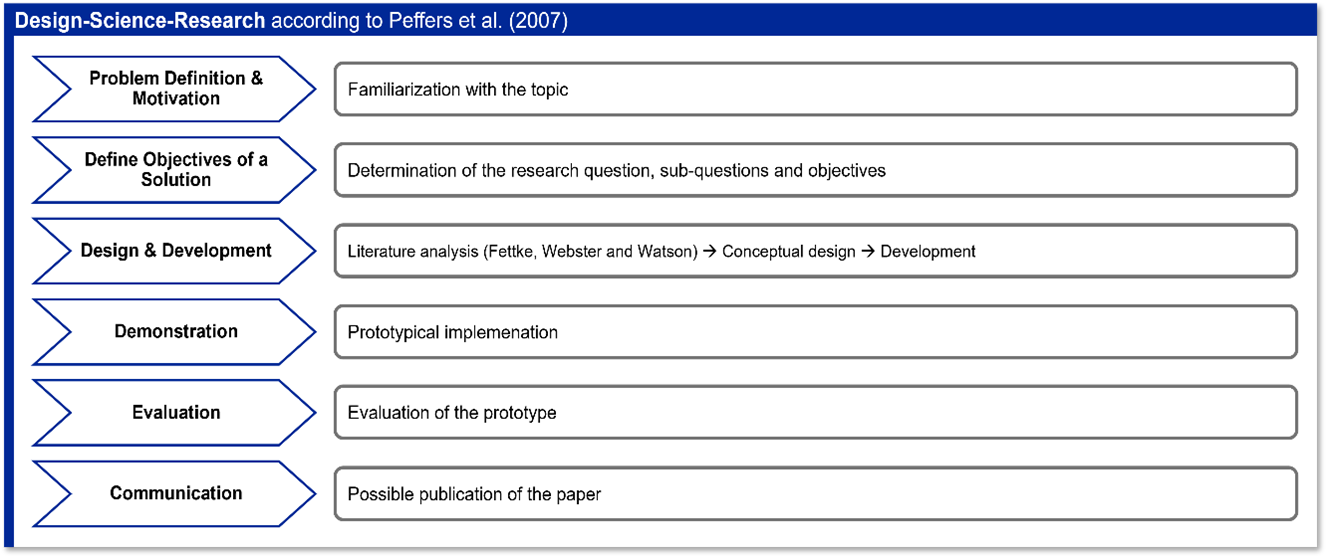
\includegraphics[width=\textwidth]{01_generalRM.png}
\caption[Overview of the general research methodology]{\label{img:generalRM}{Overview of the general research methodology \cite{peffers_design_2007}}}    
\end{figure} 

Previously, the problem upon which this work is based on and the objectives to be achieved within this work were defined in cooperation with the Frauenhofer IPA. \\

In the next steps, a comprehensive and structured literature review will be conducted with the aim of identifying the necessary foundations for GNNs, quantum computing, and the relevant molecular properties. The literature review will follow the methods of Fettke \cite{fettke_state---art_2006}, Webster and Watson \cite{webster_analyzing_2002}, as well as vom Brocke et al. \cite{vom_brocke_reconstructing_nodate}. Relevant literature databases and other elements
will be defined at the time of conducting the literature review. The results of the literature review form the first part of this work and will be documented in the form of a state-of-the-art paper.
Afterwards a classical GNN will be designed and developed to predict molecular properties using the existing data set. This serves to establish a basic understanding of GNNs and the dataset as well as possible results of the prediction. Furthermore, the classical GNN will be utilized to compare its results and performance with the quantum GNN, including various performance metrics such as accuracy.
After the successful implementation of the classical GNN, a quantum GNN will be designed and developed, which is the core focus of this thesis. The development of a quantum GNN involves using different tools and frameworks compared to a classical GNN, including the preprocessing of the available dataset. This prototype will undergo testing, evaluation, and potential optimization using a quantum computer. Specific requirements for the GNN and potential evaluation criteria will be defined as part of the research process. This can be achieved through the conducted literature review or other methods, such as expert interviews. With both classical and quantum GNNs in place, an extensive comparison between these models will be conducted. The results of this procedure constitute the second part of this thesis. The entire process and its findings will be documented.